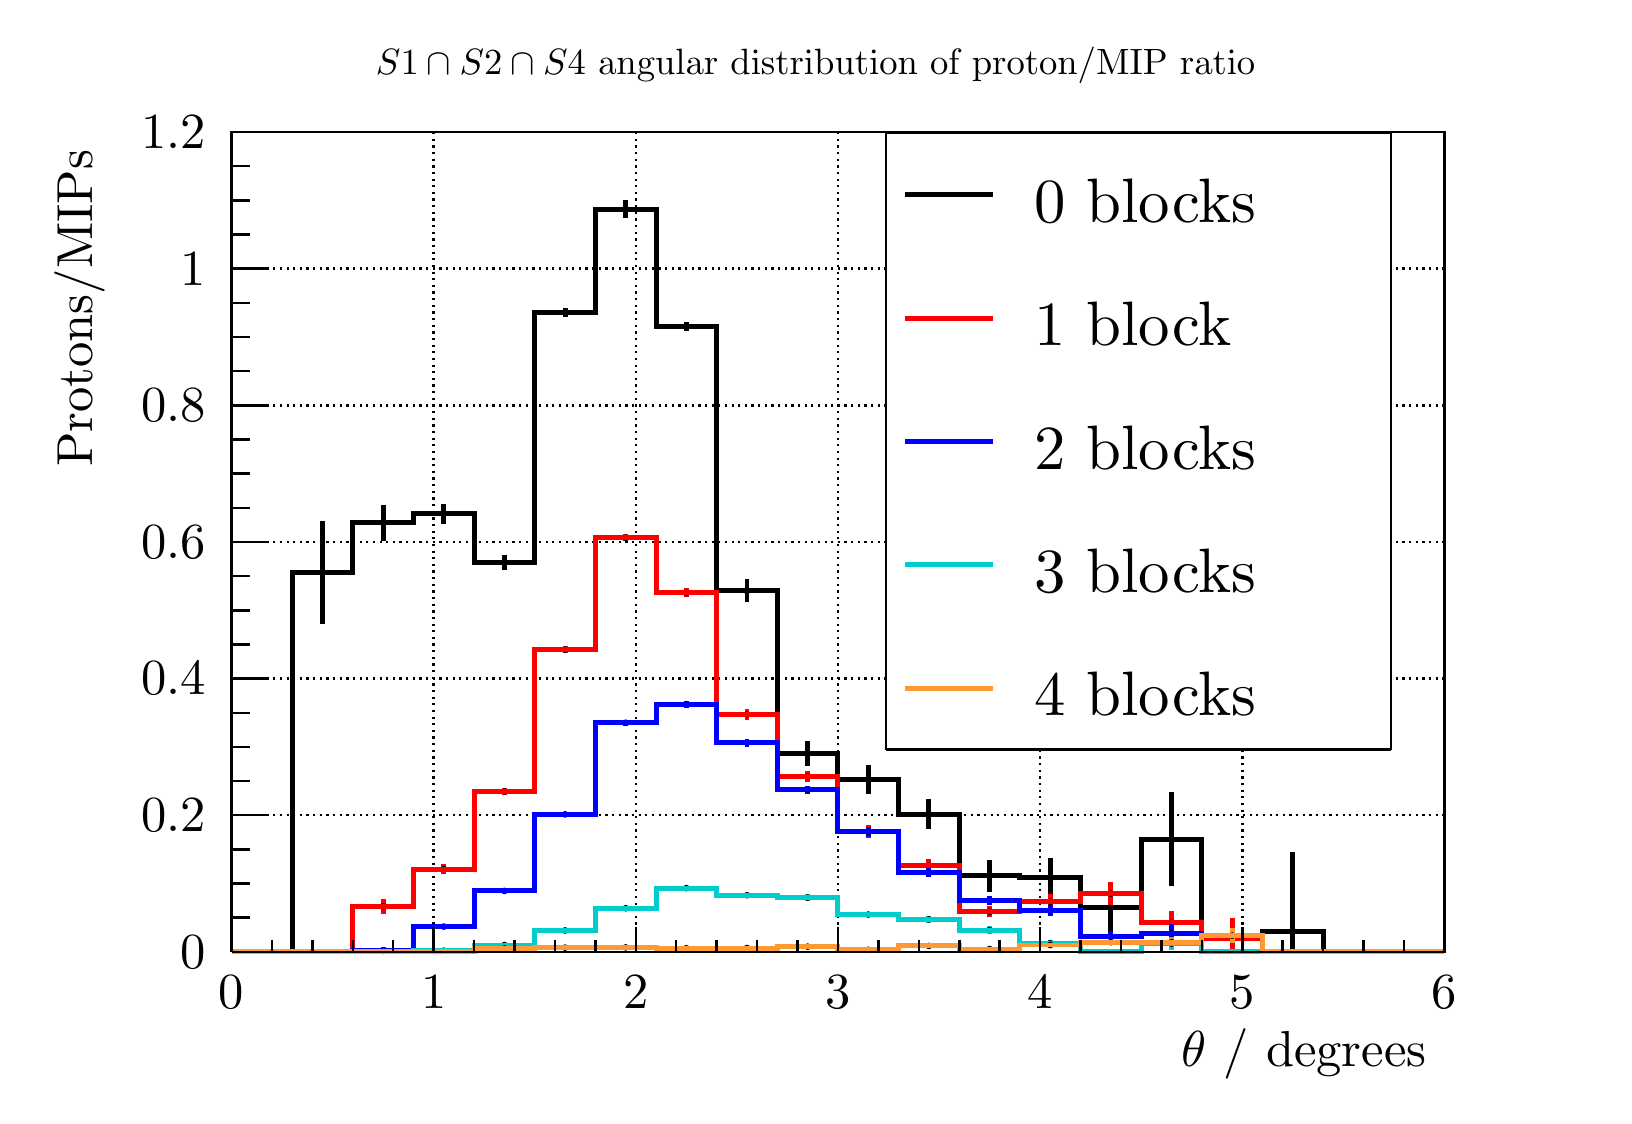
\begin{tikzpicture}
\pgfdeclareplotmark{cross} {
\pgfpathmoveto{\pgfpoint{-0.3\pgfplotmarksize}{\pgfplotmarksize}}
\pgfpathlineto{\pgfpoint{+0.3\pgfplotmarksize}{\pgfplotmarksize}}
\pgfpathlineto{\pgfpoint{+0.3\pgfplotmarksize}{0.3\pgfplotmarksize}}
\pgfpathlineto{\pgfpoint{+1\pgfplotmarksize}{0.3\pgfplotmarksize}}
\pgfpathlineto{\pgfpoint{+1\pgfplotmarksize}{-0.3\pgfplotmarksize}}
\pgfpathlineto{\pgfpoint{+0.3\pgfplotmarksize}{-0.3\pgfplotmarksize}}
\pgfpathlineto{\pgfpoint{+0.3\pgfplotmarksize}{-1.\pgfplotmarksize}}
\pgfpathlineto{\pgfpoint{-0.3\pgfplotmarksize}{-1.\pgfplotmarksize}}
\pgfpathlineto{\pgfpoint{-0.3\pgfplotmarksize}{-0.3\pgfplotmarksize}}
\pgfpathlineto{\pgfpoint{-1.\pgfplotmarksize}{-0.3\pgfplotmarksize}}
\pgfpathlineto{\pgfpoint{-1.\pgfplotmarksize}{0.3\pgfplotmarksize}}
\pgfpathlineto{\pgfpoint{-0.3\pgfplotmarksize}{0.3\pgfplotmarksize}}
\pgfpathclose
\pgfusepathqstroke
}
\pgfdeclareplotmark{cross*} {
\pgfpathmoveto{\pgfpoint{-0.3\pgfplotmarksize}{\pgfplotmarksize}}
\pgfpathlineto{\pgfpoint{+0.3\pgfplotmarksize}{\pgfplotmarksize}}
\pgfpathlineto{\pgfpoint{+0.3\pgfplotmarksize}{0.3\pgfplotmarksize}}
\pgfpathlineto{\pgfpoint{+1\pgfplotmarksize}{0.3\pgfplotmarksize}}
\pgfpathlineto{\pgfpoint{+1\pgfplotmarksize}{-0.3\pgfplotmarksize}}
\pgfpathlineto{\pgfpoint{+0.3\pgfplotmarksize}{-0.3\pgfplotmarksize}}
\pgfpathlineto{\pgfpoint{+0.3\pgfplotmarksize}{-1.\pgfplotmarksize}}
\pgfpathlineto{\pgfpoint{-0.3\pgfplotmarksize}{-1.\pgfplotmarksize}}
\pgfpathlineto{\pgfpoint{-0.3\pgfplotmarksize}{-0.3\pgfplotmarksize}}
\pgfpathlineto{\pgfpoint{-1.\pgfplotmarksize}{-0.3\pgfplotmarksize}}
\pgfpathlineto{\pgfpoint{-1.\pgfplotmarksize}{0.3\pgfplotmarksize}}
\pgfpathlineto{\pgfpoint{-0.3\pgfplotmarksize}{0.3\pgfplotmarksize}}
\pgfpathclose
\pgfusepathqfillstroke
}
\pgfdeclareplotmark{newstar} {
\pgfpathmoveto{\pgfqpoint{0pt}{\pgfplotmarksize}}
\pgfpathlineto{\pgfqpointpolar{44}{0.5\pgfplotmarksize}}
\pgfpathlineto{\pgfqpointpolar{18}{\pgfplotmarksize}}
\pgfpathlineto{\pgfqpointpolar{-20}{0.5\pgfplotmarksize}}
\pgfpathlineto{\pgfqpointpolar{-54}{\pgfplotmarksize}}
\pgfpathlineto{\pgfqpointpolar{-90}{0.5\pgfplotmarksize}}
\pgfpathlineto{\pgfqpointpolar{234}{\pgfplotmarksize}}
\pgfpathlineto{\pgfqpointpolar{198}{0.5\pgfplotmarksize}}
\pgfpathlineto{\pgfqpointpolar{162}{\pgfplotmarksize}}
\pgfpathlineto{\pgfqpointpolar{134}{0.5\pgfplotmarksize}}
\pgfpathclose
\pgfusepathqstroke
}
\pgfdeclareplotmark{newstar*} {
\pgfpathmoveto{\pgfqpoint{0pt}{\pgfplotmarksize}}
\pgfpathlineto{\pgfqpointpolar{44}{0.5\pgfplotmarksize}}
\pgfpathlineto{\pgfqpointpolar{18}{\pgfplotmarksize}}
\pgfpathlineto{\pgfqpointpolar{-20}{0.5\pgfplotmarksize}}
\pgfpathlineto{\pgfqpointpolar{-54}{\pgfplotmarksize}}
\pgfpathlineto{\pgfqpointpolar{-90}{0.5\pgfplotmarksize}}
\pgfpathlineto{\pgfqpointpolar{234}{\pgfplotmarksize}}
\pgfpathlineto{\pgfqpointpolar{198}{0.5\pgfplotmarksize}}
\pgfpathlineto{\pgfqpointpolar{162}{\pgfplotmarksize}}
\pgfpathlineto{\pgfqpointpolar{134}{0.5\pgfplotmarksize}}
\pgfpathclose
\pgfusepathqfillstroke
}
\definecolor{c}{rgb}{1,1,1};
\draw [color=c, fill=c] (0,0) rectangle (20,13.5319);
\draw [color=c, fill=c] (2.58156,1.80142) rectangle (17.9858,12.2128);
\definecolor{c}{rgb}{0,0,0};
\draw [c,line width=0.9] (2.58156,1.80142) -- (2.58156,12.2128) -- (17.9858,12.2128) -- (17.9858,1.80142) -- (2.58156,1.80142);
\definecolor{c}{rgb}{1,1,1};
\draw [color=c, fill=c] (2.58156,1.80142) rectangle (17.9858,12.2128);
\definecolor{c}{rgb}{0,0,0};
\draw [c,line width=0.9] (2.58156,1.80142) -- (2.58156,12.2128) -- (17.9858,12.2128) -- (17.9858,1.80142) -- (2.58156,1.80142);
\draw [c,line width=0.9] (2.58156,1.80142) -- (17.9858,1.80142);
\draw [c,dash pattern=on 0.80pt off 1.60pt ,line width=0.9] (2.58156,12.2128) -- (2.58156,1.80142);
\draw [c,dash pattern=on 0.80pt off 1.60pt ,line width=0.9] (5.14894,12.2128) -- (5.14894,1.80142);
\draw [c,dash pattern=on 0.80pt off 1.60pt ,line width=0.9] (7.71631,12.2128) -- (7.71631,1.80142);
\draw [c,dash pattern=on 0.80pt off 1.60pt ,line width=0.9] (10.2837,12.2128) -- (10.2837,1.80142);
\draw [c,dash pattern=on 0.80pt off 1.60pt ,line width=0.9] (12.8511,12.2128) -- (12.8511,1.80142);
\draw [c,dash pattern=on 0.80pt off 1.60pt ,line width=0.9] (15.4184,12.2128) -- (15.4184,1.80142);
\draw [c,dash pattern=on 0.80pt off 1.60pt ,line width=0.9] (17.9858,12.2128) -- (17.9858,1.80142);
\draw [c,line width=0.9] (2.58156,1.80142) -- (2.58156,12.2128);
\draw [c,dash pattern=on 0.80pt off 1.60pt ,line width=0.9] (17.9858,1.80142) -- (2.58156,1.80142);
\draw [c,dash pattern=on 0.80pt off 1.60pt ,line width=0.9] (17.9858,3.53664) -- (2.58156,3.53664);
\draw [c,dash pattern=on 0.80pt off 1.60pt ,line width=0.9] (17.9858,5.27187) -- (2.58156,5.27187);
\draw [c,dash pattern=on 0.80pt off 1.60pt ,line width=0.9] (17.9858,7.00709) -- (2.58156,7.00709);
\draw [c,dash pattern=on 0.80pt off 1.60pt ,line width=0.9] (17.9858,8.74232) -- (2.58156,8.74232);
\draw [c,dash pattern=on 0.80pt off 1.60pt ,line width=0.9] (17.9858,10.4775) -- (2.58156,10.4775);
\draw [c,dash pattern=on 0.80pt off 1.60pt ,line width=0.9] (17.9858,12.2128) -- (2.58156,12.2128);
\draw [c,dash pattern=on 0.80pt off 1.60pt ,line width=0.9] (17.9858,12.2128) -- (2.58156,12.2128);
\definecolor{c}{rgb}{0,0,0.6};
\draw [c,line width=0.9] (2.58156,1.80142) -- (3.35177,1.80142) -- (3.35177,1.80142) -- (4.12199,1.80142) -- (4.12199,1.80142) -- (4.8922,1.80142) -- (4.8922,1.80142) -- (5.66241,1.80142) -- (5.66241,1.80142) -- (6.43262,1.80142) -- (6.43262,1.80142)
 -- (7.20284,1.80142) -- (7.20284,1.80142) -- (7.97305,1.80142) -- (7.97305,1.80142) -- (8.74326,1.80142) -- (8.74326,1.80142) -- (9.51348,1.80142) -- (9.51348,1.80142) -- (10.2837,1.80142) -- (10.2837,1.80142) -- (11.0539,1.80142) --
 (11.0539,1.80142) -- (11.8241,1.80142) -- (11.8241,1.80142) -- (12.5943,1.80142) -- (12.5943,1.80142) -- (13.3645,1.80142) -- (13.3645,1.80142) -- (14.1348,1.80142) -- (14.1348,1.80142) -- (14.905,1.80142) -- (14.905,1.80142) -- (15.6752,1.80142) --
 (15.6752,1.80142) -- (16.4454,1.80142) -- (16.4454,1.80142) -- (17.2156,1.80142) -- (17.2156,1.80142) -- (17.9858,1.80142);
\definecolor{c}{rgb}{0,0,0};
\draw [c,line width=0.9] (2.58156,1.80142) -- (17.9858,1.80142);
\draw [c,line width=0.9] (2.58156,2.11409) -- (2.58156,1.80142);
\draw [c,line width=0.9] (3.09504,1.95776) -- (3.09504,1.80142);
\draw [c,line width=0.9] (3.60851,1.95776) -- (3.60851,1.80142);
\draw [c,line width=0.9] (4.12199,1.95776) -- (4.12199,1.80142);
\draw [c,line width=0.9] (4.63546,1.95776) -- (4.63546,1.80142);
\draw [c,line width=0.9] (5.14894,2.11409) -- (5.14894,1.80142);
\draw [c,line width=0.9] (5.66241,1.95776) -- (5.66241,1.80142);
\draw [c,line width=0.9] (6.17589,1.95776) -- (6.17589,1.80142);
\draw [c,line width=0.9] (6.68936,1.95776) -- (6.68936,1.80142);
\draw [c,line width=0.9] (7.20284,1.95776) -- (7.20284,1.80142);
\draw [c,line width=0.9] (7.71631,2.11409) -- (7.71631,1.80142);
\draw [c,line width=0.9] (8.22979,1.95776) -- (8.22979,1.80142);
\draw [c,line width=0.9] (8.74326,1.95776) -- (8.74326,1.80142);
\draw [c,line width=0.9] (9.25674,1.95776) -- (9.25674,1.80142);
\draw [c,line width=0.9] (9.77021,1.95776) -- (9.77021,1.80142);
\draw [c,line width=0.9] (10.2837,2.11409) -- (10.2837,1.80142);
\draw [c,line width=0.9] (10.7972,1.95776) -- (10.7972,1.80142);
\draw [c,line width=0.9] (11.3106,1.95776) -- (11.3106,1.80142);
\draw [c,line width=0.9] (11.8241,1.95776) -- (11.8241,1.80142);
\draw [c,line width=0.9] (12.3376,1.95776) -- (12.3376,1.80142);
\draw [c,line width=0.9] (12.8511,2.11409) -- (12.8511,1.80142);
\draw [c,line width=0.9] (13.3645,1.95776) -- (13.3645,1.80142);
\draw [c,line width=0.9] (13.878,1.95776) -- (13.878,1.80142);
\draw [c,line width=0.9] (14.3915,1.95776) -- (14.3915,1.80142);
\draw [c,line width=0.9] (14.905,1.95776) -- (14.905,1.80142);
\draw [c,line width=0.9] (15.4184,2.11409) -- (15.4184,1.80142);
\draw [c,line width=0.9] (15.9319,1.95776) -- (15.9319,1.80142);
\draw [c,line width=0.9] (16.4454,1.95776) -- (16.4454,1.80142);
\draw [c,line width=0.9] (16.9589,1.95776) -- (16.9589,1.80142);
\draw [c,line width=0.9] (17.4723,1.95776) -- (17.4723,1.80142);
\draw [c,line width=0.9] (17.9858,2.11409) -- (17.9858,1.80142);
\draw [anchor=base] (2.58156,1.08423) node[scale=1.82718, color=c, rotate=0]{0};
\draw [anchor=base] (5.14894,1.08423) node[scale=1.82718, color=c, rotate=0]{1};
\draw [anchor=base] (7.71631,1.08423) node[scale=1.82718, color=c, rotate=0]{2};
\draw [anchor=base] (10.2837,1.08423) node[scale=1.82718, color=c, rotate=0]{3};
\draw [anchor=base] (12.8511,1.08423) node[scale=1.82718, color=c, rotate=0]{4};
\draw [anchor=base] (15.4184,1.08423) node[scale=1.82718, color=c, rotate=0]{5};
\draw [anchor=base] (17.9858,1.08423) node[scale=1.82718, color=c, rotate=0]{6};
\draw [anchor= east] (17.9858,0.502355) node[scale=1.82718, color=c, rotate=0]{$\theta$ / degrees};
\draw [c,line width=0.9] (2.58156,1.80142) -- (2.58156,12.2128);
\draw [c,line width=0.9] (3.0432,1.80142) -- (2.58156,1.80142);
\draw [c,line width=0.9] (2.81238,2.23522) -- (2.58156,2.23522);
\draw [c,line width=0.9] (2.81238,2.66903) -- (2.58156,2.66903);
\draw [c,line width=0.9] (2.81238,3.10284) -- (2.58156,3.10284);
\draw [c,line width=0.9] (3.0432,3.53664) -- (2.58156,3.53664);
\draw [c,line width=0.9] (2.81238,3.97045) -- (2.58156,3.97045);
\draw [c,line width=0.9] (2.81238,4.40426) -- (2.58156,4.40426);
\draw [c,line width=0.9] (2.81238,4.83806) -- (2.58156,4.83806);
\draw [c,line width=0.9] (3.0432,5.27187) -- (2.58156,5.27187);
\draw [c,line width=0.9] (2.81238,5.70567) -- (2.58156,5.70567);
\draw [c,line width=0.9] (2.81238,6.13948) -- (2.58156,6.13948);
\draw [c,line width=0.9] (2.81238,6.57329) -- (2.58156,6.57329);
\draw [c,line width=0.9] (3.0432,7.00709) -- (2.58156,7.00709);
\draw [c,line width=0.9] (2.81238,7.4409) -- (2.58156,7.4409);
\draw [c,line width=0.9] (2.81238,7.8747) -- (2.58156,7.8747);
\draw [c,line width=0.9] (2.81238,8.30851) -- (2.58156,8.30851);
\draw [c,line width=0.9] (3.0432,8.74232) -- (2.58156,8.74232);
\draw [c,line width=0.9] (2.81238,9.17612) -- (2.58156,9.17612);
\draw [c,line width=0.9] (2.81238,9.60993) -- (2.58156,9.60993);
\draw [c,line width=0.9] (2.81238,10.0437) -- (2.58156,10.0437);
\draw [c,line width=0.9] (3.0432,10.4775) -- (2.58156,10.4775);
\draw [c,line width=0.9] (2.81238,10.9113) -- (2.58156,10.9113);
\draw [c,line width=0.9] (2.81238,11.3452) -- (2.58156,11.3452);
\draw [c,line width=0.9] (2.81238,11.779) -- (2.58156,11.779);
\draw [c,line width=0.9] (3.0432,12.2128) -- (2.58156,12.2128);
\draw [c,line width=0.9] (3.0432,12.2128) -- (2.58156,12.2128);
\draw [anchor= east] (2.48156,1.80142) node[scale=1.82718, color=c, rotate=0]{0};
\draw [anchor= east] (2.48156,3.53664) node[scale=1.82718, color=c, rotate=0]{0.2};
\draw [anchor= east] (2.48156,5.27187) node[scale=1.82718, color=c, rotate=0]{0.4};
\draw [anchor= east] (2.48156,7.00709) node[scale=1.82718, color=c, rotate=0]{0.6};
\draw [anchor= east] (2.48156,8.74232) node[scale=1.82718, color=c, rotate=0]{0.8};
\draw [anchor= east] (2.48156,10.4775) node[scale=1.82718, color=c, rotate=0]{1};
\draw [anchor= east] (2.48156,12.2128) node[scale=1.82718, color=c, rotate=0]{1.2};
\draw [anchor= east] (0.66156,12.2128) node[scale=1.82718, color=c, rotate=90]{ Protons/MIPs};
\draw [c,line width=1.8] (3.73688,5.96909) -- (3.73688,6.61835);
\draw [c,line width=1.8] (3.73688,6.61835) -- (3.73688,7.26762);
\foreach \P in {(3.73688,6.61835)}{\draw[mark options={color=c,fill=c},mark size=2.402402pt,mark=*,mark size=1pt] plot coordinates {\P};}
\draw [c,line width=1.8] (4.50709,7.01665) -- (4.50709,7.24975);
\draw [c,line width=1.8] (4.50709,7.24975) -- (4.50709,7.48286);
\foreach \P in {(4.50709,7.24975)}{\draw[mark options={color=c,fill=c},mark size=2.402402pt,mark=*,mark size=1pt] plot coordinates {\P};}
\draw [c,line width=1.8] (5.27731,7.23951) -- (5.27731,7.36405);
\draw [c,line width=1.8] (5.27731,7.36405) -- (5.27731,7.4886);
\foreach \P in {(5.27731,7.36405)}{\draw[mark options={color=c,fill=c},mark size=2.402402pt,mark=*,mark size=1pt] plot coordinates {\P};}
\draw [c,line width=1.8] (6.04752,6.65693) -- (6.04752,6.75156);
\draw [c,line width=1.8] (6.04752,6.75156) -- (6.04752,6.8462);
\foreach \P in {(6.04752,6.75156)}{\draw[mark options={color=c,fill=c},mark size=2.402402pt,mark=*,mark size=1pt] plot coordinates {\P};}
\draw [c,line width=1.8] (6.81773,9.86403) -- (6.81773,9.92111);
\draw [c,line width=1.8] (6.81773,9.92111) -- (6.81773,9.97818);
\foreach \P in {(6.81773,9.92111)}{\draw[mark options={color=c,fill=c},mark size=2.402402pt,mark=*,mark size=1pt] plot coordinates {\P};}
\draw [c,line width=1.8] (7.58794,11.1257) -- (7.58794,11.2349);
\draw [c,line width=1.8] (7.58794,11.2349) -- (7.58794,11.3441);
\foreach \P in {(7.58794,11.2349)}{\draw[mark options={color=c,fill=c},mark size=2.402402pt,mark=*,mark size=1pt] plot coordinates {\P};}
\draw [c,line width=1.8] (8.35816,9.68957) -- (8.35816,9.74459);
\draw [c,line width=1.8] (8.35816,9.74459) -- (8.35816,9.7996);
\foreach \P in {(8.35816,9.74459)}{\draw[mark options={color=c,fill=c},mark size=2.402402pt,mark=*,mark size=1pt] plot coordinates {\P};}
\draw [c,line width=1.8] (9.12837,6.24154) -- (9.12837,6.38654);
\draw [c,line width=1.8] (9.12837,6.38654) -- (9.12837,6.53154);
\foreach \P in {(9.12837,6.38654)}{\draw[mark options={color=c,fill=c},mark size=2.402402pt,mark=*,mark size=1pt] plot coordinates {\P};}
\draw [c,line width=1.8] (9.89858,4.16117) -- (9.89858,4.3187);
\draw [c,line width=1.8] (9.89858,4.3187) -- (9.89858,4.47623);
\foreach \P in {(9.89858,4.3187)}{\draw[mark options={color=c,fill=c},mark size=2.402402pt,mark=*,mark size=1pt] plot coordinates {\P};}
\draw [c,line width=1.8] (10.6688,3.80166) -- (10.6688,3.99015);
\draw [c,line width=1.8] (10.6688,3.99015) -- (10.6688,4.17865);
\foreach \P in {(10.6688,3.99015)}{\draw[mark options={color=c,fill=c},mark size=2.402402pt,mark=*,mark size=1pt] plot coordinates {\P};}
\draw [c,line width=1.8] (11.439,3.36091) -- (11.439,3.55216);
\draw [c,line width=1.8] (11.439,3.55216) -- (11.439,3.7434);
\foreach \P in {(11.439,3.55216)}{\draw[mark options={color=c,fill=c},mark size=2.402402pt,mark=*,mark size=1pt] plot coordinates {\P};}
\draw [c,line width=1.8] (12.2092,2.56466) -- (12.2092,2.76596);
\draw [c,line width=1.8] (12.2092,2.76596) -- (12.2092,2.96726);
\foreach \P in {(12.2092,2.76596)}{\draw[mark options={color=c,fill=c},mark size=2.402402pt,mark=*,mark size=1pt] plot coordinates {\P};}
\draw [c,line width=1.8] (12.9794,2.50973) -- (12.9794,2.75162);
\draw [c,line width=1.8] (12.9794,2.75162) -- (12.9794,2.9935);
\foreach \P in {(12.9794,2.75162)}{\draw[mark options={color=c,fill=c},mark size=2.402402pt,mark=*,mark size=1pt] plot coordinates {\P};}
\draw [c,line width=1.8] (13.7496,2.0489) -- (13.7496,2.36584);
\draw [c,line width=1.8] (13.7496,2.36584) -- (13.7496,2.68279);
\foreach \P in {(13.7496,2.36584)}{\draw[mark options={color=c,fill=c},mark size=2.402402pt,mark=*,mark size=1pt] plot coordinates {\P};}
\draw [c,line width=1.8] (14.5199,2.63323) -- (14.5199,3.23146);
\draw [c,line width=1.8] (14.5199,3.23146) -- (14.5199,3.82969);
\foreach \P in {(14.5199,3.23146)}{\draw[mark options={color=c,fill=c},mark size=2.402402pt,mark=*,mark size=1pt] plot coordinates {\P};}
\draw [c,line width=1.8] (16.0603,1.80142) -- (16.0603,2.06459);
\draw [c,line width=1.8] (16.0603,2.06459) -- (16.0603,3.06406);
\foreach \P in {(16.0603,2.06459)}{\draw[mark options={color=c,fill=c},mark size=2.402402pt,mark=*,mark size=1pt] plot coordinates {\P};}
\draw [c,line width=1.8] (2.58156,1.80142) -- (3.35177,1.80142) -- (3.35177,6.61835) -- (4.12199,6.61835) -- (4.12199,7.24975) -- (4.8922,7.24975) -- (4.8922,7.36405) -- (5.66241,7.36405) -- (5.66241,6.75156) -- (6.43262,6.75156) -- (6.43262,9.92111)
 -- (7.20284,9.92111) -- (7.20284,11.2349) -- (7.97305,11.2349) -- (7.97305,9.74459) -- (8.74326,9.74459) -- (8.74326,6.38654) -- (9.51348,6.38654) -- (9.51348,4.3187) -- (10.2837,4.3187) -- (10.2837,3.99015) -- (11.0539,3.99015) -- (11.0539,3.55216)
 -- (11.8241,3.55216) -- (11.8241,2.76596) -- (12.5943,2.76596) -- (12.5943,2.75162) -- (13.3645,2.75162) -- (13.3645,2.36584) -- (14.1348,2.36584) -- (14.1348,3.23146) -- (14.905,3.23146) -- (14.905,1.80142) -- (15.6752,1.80142) -- (15.6752,2.06459)
 -- (16.4454,2.06459) -- (16.4454,1.80142) -- (17.2156,1.80142) -- (17.2156,1.80142) -- (17.9858,1.80142);
\definecolor{c}{rgb}{1,0,0};
\draw [c,line width=1.8] (4.50709,2.28567) -- (4.50709,2.37944);
\draw [c,line width=1.8] (4.50709,2.37944) -- (4.50709,2.47322);
\definecolor{c}{rgb}{0,0,0};
\foreach \P in {(4.50709,2.37944)}{\draw[mark options={color=c,fill=c},mark size=2.402402pt,mark=*,mark size=1pt] plot coordinates {\P};}
\definecolor{c}{rgb}{1,0,0};
\draw [c,line width=1.8] (5.27731,2.79594) -- (5.27731,2.85369);
\draw [c,line width=1.8] (5.27731,2.85369) -- (5.27731,2.91144);
\definecolor{c}{rgb}{0,0,0};
\foreach \P in {(5.27731,2.85369)}{\draw[mark options={color=c,fill=c},mark size=2.402402pt,mark=*,mark size=1pt] plot coordinates {\P};}
\definecolor{c}{rgb}{1,0,0};
\draw [c,line width=1.8] (6.04752,3.79475) -- (6.04752,3.8403);
\draw [c,line width=1.8] (6.04752,3.8403) -- (6.04752,3.88585);
\definecolor{c}{rgb}{0,0,0};
\foreach \P in {(6.04752,3.8403)}{\draw[mark options={color=c,fill=c},mark size=2.402402pt,mark=*,mark size=1pt] plot coordinates {\P};}
\definecolor{c}{rgb}{1,0,0};
\draw [c,line width=1.8] (6.81773,5.59646) -- (6.81773,5.64017);
\draw [c,line width=1.8] (6.81773,5.64017) -- (6.81773,5.68388);
\definecolor{c}{rgb}{0,0,0};
\foreach \P in {(6.81773,5.64017)}{\draw[mark options={color=c,fill=c},mark size=2.402402pt,mark=*,mark size=1pt] plot coordinates {\P};}
\definecolor{c}{rgb}{1,0,0};
\draw [c,line width=1.8] (7.58794,7.01498) -- (7.58794,7.05941);
\draw [c,line width=1.8] (7.58794,7.05941) -- (7.58794,7.10384);
\definecolor{c}{rgb}{0,0,0};
\foreach \P in {(7.58794,7.05941)}{\draw[mark options={color=c,fill=c},mark size=2.402402pt,mark=*,mark size=1pt] plot coordinates {\P};}
\definecolor{c}{rgb}{1,0,0};
\draw [c,line width=1.8] (8.35816,6.30632) -- (8.35816,6.36152);
\draw [c,line width=1.8] (8.35816,6.36152) -- (8.35816,6.41672);
\definecolor{c}{rgb}{0,0,0};
\foreach \P in {(8.35816,6.36152)}{\draw[mark options={color=c,fill=c},mark size=2.402402pt,mark=*,mark size=1pt] plot coordinates {\P};}
\definecolor{c}{rgb}{1,0,0};
\draw [c,line width=1.8] (9.12837,4.74977) -- (9.12837,4.81839);
\draw [c,line width=1.8] (9.12837,4.81839) -- (9.12837,4.88701);
\definecolor{c}{rgb}{0,0,0};
\foreach \P in {(9.12837,4.81839)}{\draw[mark options={color=c,fill=c},mark size=2.402402pt,mark=*,mark size=1pt] plot coordinates {\P};}
\definecolor{c}{rgb}{1,0,0};
\draw [c,line width=1.8] (9.89858,3.95546) -- (9.89858,4.03007);
\draw [c,line width=1.8] (9.89858,4.03007) -- (9.89858,4.10467);
\definecolor{c}{rgb}{0,0,0};
\foreach \P in {(9.89858,4.03007)}{\draw[mark options={color=c,fill=c},mark size=2.402402pt,mark=*,mark size=1pt] plot coordinates {\P};}
\definecolor{c}{rgb}{1,0,0};
\draw [c,line width=1.8] (10.6688,3.24766) -- (10.6688,3.32829);
\draw [c,line width=1.8] (10.6688,3.32829) -- (10.6688,3.40892);
\definecolor{c}{rgb}{0,0,0};
\foreach \P in {(10.6688,3.32829)}{\draw[mark options={color=c,fill=c},mark size=2.402402pt,mark=*,mark size=1pt] plot coordinates {\P};}
\definecolor{c}{rgb}{1,0,0};
\draw [c,line width=1.8] (11.439,2.81238) -- (11.439,2.89504);
\draw [c,line width=1.8] (11.439,2.89504) -- (11.439,2.97769);
\definecolor{c}{rgb}{0,0,0};
\foreach \P in {(11.439,2.89504)}{\draw[mark options={color=c,fill=c},mark size=2.402402pt,mark=*,mark size=1pt] plot coordinates {\P};}
\definecolor{c}{rgb}{1,0,0};
\draw [c,line width=1.8] (12.2092,2.24132) -- (12.2092,2.31194);
\draw [c,line width=1.8] (12.2092,2.31194) -- (12.2092,2.38256);
\definecolor{c}{rgb}{0,0,0};
\foreach \P in {(12.2092,2.31194)}{\draw[mark options={color=c,fill=c},mark size=2.402402pt,mark=*,mark size=1pt] plot coordinates {\P};}
\definecolor{c}{rgb}{1,0,0};
\draw [c,line width=1.8] (12.9794,2.33711) -- (12.9794,2.43758);
\draw [c,line width=1.8] (12.9794,2.43758) -- (12.9794,2.53805);
\definecolor{c}{rgb}{0,0,0};
\foreach \P in {(12.9794,2.43758)}{\draw[mark options={color=c,fill=c},mark size=2.402402pt,mark=*,mark size=1pt] plot coordinates {\P};}
\definecolor{c}{rgb}{1,0,0};
\draw [c,line width=1.8] (13.7496,2.39958) -- (13.7496,2.54141);
\draw [c,line width=1.8] (13.7496,2.54141) -- (13.7496,2.68324);
\definecolor{c}{rgb}{0,0,0};
\foreach \P in {(13.7496,2.54141)}{\draw[mark options={color=c,fill=c},mark size=2.402402pt,mark=*,mark size=1pt] plot coordinates {\P};}
\definecolor{c}{rgb}{1,0,0};
\draw [c,line width=1.8] (14.5199,2.01609) -- (14.5199,2.17081);
\draw [c,line width=1.8] (14.5199,2.17081) -- (14.5199,2.32553);
\definecolor{c}{rgb}{0,0,0};
\foreach \P in {(14.5199,2.17081)}{\draw[mark options={color=c,fill=c},mark size=2.402402pt,mark=*,mark size=1pt] plot coordinates {\P};}
\definecolor{c}{rgb}{1,0,0};
\draw [c,line width=1.8] (15.2901,1.80142) -- (15.2901,1.9743);
\draw [c,line width=1.8] (15.2901,1.9743) -- (15.2901,2.22633);
\definecolor{c}{rgb}{0,0,0};
\foreach \P in {(15.2901,1.9743)}{\draw[mark options={color=c,fill=c},mark size=2.402402pt,mark=*,mark size=1pt] plot coordinates {\P};}
\definecolor{c}{rgb}{1,0,0};
\draw [c,line width=1.8] (2.58156,1.80142) -- (3.35177,1.80142) -- (3.35177,1.80142) -- (4.12199,1.80142) -- (4.12199,2.37944) -- (4.8922,2.37944) -- (4.8922,2.85369) -- (5.66241,2.85369) -- (5.66241,3.8403) -- (6.43262,3.8403) -- (6.43262,5.64017)
 -- (7.20284,5.64017) -- (7.20284,7.05941) -- (7.97305,7.05941) -- (7.97305,6.36152) -- (8.74326,6.36152) -- (8.74326,4.81839) -- (9.51348,4.81839) -- (9.51348,4.03007) -- (10.2837,4.03007) -- (10.2837,3.32829) -- (11.0539,3.32829) --
 (11.0539,2.89504) -- (11.8241,2.89504) -- (11.8241,2.31194) -- (12.5943,2.31194) -- (12.5943,2.43758) -- (13.3645,2.43758) -- (13.3645,2.54141) -- (14.1348,2.54141) -- (14.1348,2.17081) -- (14.905,2.17081) -- (14.905,1.9743) -- (15.6752,1.9743) --
 (15.6752,1.80142) -- (16.4454,1.80142) -- (16.4454,1.80142) -- (17.2156,1.80142) -- (17.2156,1.80142) -- (17.9858,1.80142);
\definecolor{c}{rgb}{0,0,1};
\draw [c,line width=1.8] (4.50709,1.80142) -- (4.50709,1.81398);
\draw [c,line width=1.8] (4.50709,1.81398) -- (4.50709,1.86696);
\definecolor{c}{rgb}{0,0,0};
\foreach \P in {(4.50709,1.81398)}{\draw[mark options={color=c,fill=c},mark size=2.402402pt,mark=*,mark size=1pt] plot coordinates {\P};}
\definecolor{c}{rgb}{0,0,1};
\draw [c,line width=1.8] (5.27731,2.09007) -- (5.27731,2.12258);
\draw [c,line width=1.8] (5.27731,2.12258) -- (5.27731,2.15509);
\definecolor{c}{rgb}{0,0,0};
\foreach \P in {(5.27731,2.12258)}{\draw[mark options={color=c,fill=c},mark size=2.402402pt,mark=*,mark size=1pt] plot coordinates {\P};}
\definecolor{c}{rgb}{0,0,1};
\draw [c,line width=1.8] (6.04752,2.54822) -- (6.04752,2.57576);
\draw [c,line width=1.8] (6.04752,2.57576) -- (6.04752,2.60329);
\definecolor{c}{rgb}{0,0,0};
\foreach \P in {(6.04752,2.57576)}{\draw[mark options={color=c,fill=c},mark size=2.402402pt,mark=*,mark size=1pt] plot coordinates {\P};}
\definecolor{c}{rgb}{0,0,1};
\draw [c,line width=1.8] (6.81773,3.51697) -- (6.81773,3.54787);
\draw [c,line width=1.8] (6.81773,3.54787) -- (6.81773,3.57877);
\definecolor{c}{rgb}{0,0,0};
\foreach \P in {(6.81773,3.54787)}{\draw[mark options={color=c,fill=c},mark size=2.402402pt,mark=*,mark size=1pt] plot coordinates {\P};}
\definecolor{c}{rgb}{0,0,1};
\draw [c,line width=1.8] (7.58794,4.67507) -- (7.58794,4.71136);
\draw [c,line width=1.8] (7.58794,4.71136) -- (7.58794,4.74765);
\definecolor{c}{rgb}{0,0,0};
\foreach \P in {(7.58794,4.71136)}{\draw[mark options={color=c,fill=c},mark size=2.402402pt,mark=*,mark size=1pt] plot coordinates {\P};}
\definecolor{c}{rgb}{0,0,1};
\draw [c,line width=1.8] (8.35816,4.90264) -- (8.35816,4.94582);
\draw [c,line width=1.8] (8.35816,4.94582) -- (8.35816,4.989);
\definecolor{c}{rgb}{0,0,0};
\foreach \P in {(8.35816,4.94582)}{\draw[mark options={color=c,fill=c},mark size=2.402402pt,mark=*,mark size=1pt] plot coordinates {\P};}
\definecolor{c}{rgb}{0,0,1};
\draw [c,line width=1.8] (9.12837,4.40846) -- (9.12837,4.45857);
\draw [c,line width=1.8] (9.12837,4.45857) -- (9.12837,4.50869);
\definecolor{c}{rgb}{0,0,0};
\foreach \P in {(9.12837,4.45857)}{\draw[mark options={color=c,fill=c},mark size=2.402402pt,mark=*,mark size=1pt] plot coordinates {\P};}
\definecolor{c}{rgb}{0,0,1};
\draw [c,line width=1.8] (9.89858,3.80403) -- (9.89858,3.85863);
\draw [c,line width=1.8] (9.89858,3.85863) -- (9.89858,3.91322);
\definecolor{c}{rgb}{0,0,0};
\foreach \P in {(9.89858,3.85863)}{\draw[mark options={color=c,fill=c},mark size=2.402402pt,mark=*,mark size=1pt] plot coordinates {\P};}
\definecolor{c}{rgb}{0,0,1};
\draw [c,line width=1.8] (10.6688,3.26646) -- (10.6688,3.32506);
\draw [c,line width=1.8] (10.6688,3.32506) -- (10.6688,3.38365);
\definecolor{c}{rgb}{0,0,0};
\foreach \P in {(10.6688,3.32506)}{\draw[mark options={color=c,fill=c},mark size=2.402402pt,mark=*,mark size=1pt] plot coordinates {\P};}
\definecolor{c}{rgb}{0,0,1};
\draw [c,line width=1.8] (11.439,2.74672) -- (11.439,2.80496);
\draw [c,line width=1.8] (11.439,2.80496) -- (11.439,2.86321);
\definecolor{c}{rgb}{0,0,0};
\foreach \P in {(11.439,2.80496)}{\draw[mark options={color=c,fill=c},mark size=2.402402pt,mark=*,mark size=1pt] plot coordinates {\P};}
\definecolor{c}{rgb}{0,0,1};
\draw [c,line width=1.8] (12.2092,2.39395) -- (12.2092,2.45466);
\draw [c,line width=1.8] (12.2092,2.45466) -- (12.2092,2.51538);
\definecolor{c}{rgb}{0,0,0};
\foreach \P in {(12.2092,2.45466)}{\draw[mark options={color=c,fill=c},mark size=2.402402pt,mark=*,mark size=1pt] plot coordinates {\P};}
\definecolor{c}{rgb}{0,0,1};
\draw [c,line width=1.8] (12.9794,2.25451) -- (12.9794,2.3228);
\draw [c,line width=1.8] (12.9794,2.3228) -- (12.9794,2.3911);
\definecolor{c}{rgb}{0,0,0};
\foreach \P in {(12.9794,2.3228)}{\draw[mark options={color=c,fill=c},mark size=2.402402pt,mark=*,mark size=1pt] plot coordinates {\P};}
\definecolor{c}{rgb}{0,0,1};
\draw [c,line width=1.8] (13.7496,1.91894) -- (13.7496,1.99469);
\draw [c,line width=1.8] (13.7496,1.99469) -- (13.7496,2.07043);
\definecolor{c}{rgb}{0,0,0};
\foreach \P in {(13.7496,1.99469)}{\draw[mark options={color=c,fill=c},mark size=2.402402pt,mark=*,mark size=1pt] plot coordinates {\P};}
\definecolor{c}{rgb}{0,0,1};
\draw [c,line width=1.8] (14.5199,1.91933) -- (14.5199,2.03567);
\draw [c,line width=1.8] (14.5199,2.03567) -- (14.5199,2.152);
\definecolor{c}{rgb}{0,0,0};
\foreach \P in {(14.5199,2.03567)}{\draw[mark options={color=c,fill=c},mark size=2.402402pt,mark=*,mark size=1pt] plot coordinates {\P};}
\definecolor{c}{rgb}{0,0,1};
\draw [c,line width=1.8] (2.58156,1.80142) -- (3.35177,1.80142) -- (3.35177,1.80142) -- (4.12199,1.80142) -- (4.12199,1.81398) -- (4.8922,1.81398) -- (4.8922,2.12258) -- (5.66241,2.12258) -- (5.66241,2.57576) -- (6.43262,2.57576) -- (6.43262,3.54787)
 -- (7.20284,3.54787) -- (7.20284,4.71136) -- (7.97305,4.71136) -- (7.97305,4.94582) -- (8.74326,4.94582) -- (8.74326,4.45857) -- (9.51348,4.45857) -- (9.51348,3.85863) -- (10.2837,3.85863) -- (10.2837,3.32506) -- (11.0539,3.32506) --
 (11.0539,2.80496) -- (11.8241,2.80496) -- (11.8241,2.45466) -- (12.5943,2.45466) -- (12.5943,2.3228) -- (13.3645,2.3228) -- (13.3645,1.99469) -- (14.1348,1.99469) -- (14.1348,2.03567) -- (14.905,2.03567) -- (14.905,1.80142) -- (15.6752,1.80142) --
 (15.6752,1.80142) -- (16.4454,1.80142) -- (16.4454,1.80142) -- (17.2156,1.80142) -- (17.2156,1.80142) -- (17.9858,1.80142);
\definecolor{c}{rgb}{0,0.8,0.8};
\draw [c,line width=1.8] (5.27731,1.80142) -- (5.27731,1.81623);
\draw [c,line width=1.8] (5.27731,1.81623) -- (5.27731,1.83425);
\definecolor{c}{rgb}{0,0,0};
\foreach \P in {(5.27731,1.81623)}{\draw[mark options={color=c,fill=c},mark size=2.402402pt,mark=*,mark size=1pt] plot coordinates {\P};}
\definecolor{c}{rgb}{0,0.8,0.8};
\draw [c,line width=1.8] (6.04752,1.87586) -- (6.04752,1.88848);
\draw [c,line width=1.8] (6.04752,1.88848) -- (6.04752,1.90109);
\definecolor{c}{rgb}{0,0,0};
\foreach \P in {(6.04752,1.88848)}{\draw[mark options={color=c,fill=c},mark size=2.402402pt,mark=*,mark size=1pt] plot coordinates {\P};}
\definecolor{c}{rgb}{0,0.8,0.8};
\draw [c,line width=1.8] (6.81773,2.05676) -- (6.81773,2.07357);
\draw [c,line width=1.8] (6.81773,2.07357) -- (6.81773,2.09039);
\definecolor{c}{rgb}{0,0,0};
\foreach \P in {(6.81773,2.07357)}{\draw[mark options={color=c,fill=c},mark size=2.402402pt,mark=*,mark size=1pt] plot coordinates {\P};}
\definecolor{c}{rgb}{0,0.8,0.8};
\draw [c,line width=1.8] (7.58794,2.33449) -- (7.58794,2.3559);
\draw [c,line width=1.8] (7.58794,2.3559) -- (7.58794,2.37732);
\definecolor{c}{rgb}{0,0,0};
\foreach \P in {(7.58794,2.3559)}{\draw[mark options={color=c,fill=c},mark size=2.402402pt,mark=*,mark size=1pt] plot coordinates {\P};}
\definecolor{c}{rgb}{0,0.8,0.8};
\draw [c,line width=1.8] (8.35816,2.58185) -- (8.35816,2.61084);
\draw [c,line width=1.8] (8.35816,2.61084) -- (8.35816,2.63983);
\definecolor{c}{rgb}{0,0,0};
\foreach \P in {(8.35816,2.61084)}{\draw[mark options={color=c,fill=c},mark size=2.402402pt,mark=*,mark size=1pt] plot coordinates {\P};}
\definecolor{c}{rgb}{0,0.8,0.8};
\draw [c,line width=1.8] (9.12837,2.48791) -- (9.12837,2.52137);
\draw [c,line width=1.8] (9.12837,2.52137) -- (9.12837,2.55483);
\definecolor{c}{rgb}{0,0,0};
\foreach \P in {(9.12837,2.52137)}{\draw[mark options={color=c,fill=c},mark size=2.402402pt,mark=*,mark size=1pt] plot coordinates {\P};}
\definecolor{c}{rgb}{0,0.8,0.8};
\draw [c,line width=1.8] (9.89858,2.45146) -- (9.89858,2.49097);
\draw [c,line width=1.8] (9.89858,2.49097) -- (9.89858,2.53049);
\definecolor{c}{rgb}{0,0,0};
\foreach \P in {(9.89858,2.49097)}{\draw[mark options={color=c,fill=c},mark size=2.402402pt,mark=*,mark size=1pt] plot coordinates {\P};}
\definecolor{c}{rgb}{0,0.8,0.8};
\draw [c,line width=1.8] (10.6688,2.23827) -- (10.6688,2.27536);
\draw [c,line width=1.8] (10.6688,2.27536) -- (10.6688,2.31244);
\definecolor{c}{rgb}{0,0,0};
\foreach \P in {(10.6688,2.27536)}{\draw[mark options={color=c,fill=c},mark size=2.402402pt,mark=*,mark size=1pt] plot coordinates {\P};}
\definecolor{c}{rgb}{0,0.8,0.8};
\draw [c,line width=1.8] (11.439,2.17384) -- (11.439,2.2146);
\draw [c,line width=1.8] (11.439,2.2146) -- (11.439,2.25536);
\definecolor{c}{rgb}{0,0,0};
\foreach \P in {(11.439,2.2146)}{\draw[mark options={color=c,fill=c},mark size=2.402402pt,mark=*,mark size=1pt] plot coordinates {\P};}
\definecolor{c}{rgb}{0,0.8,0.8};
\draw [c,line width=1.8] (12.2092,2.03257) -- (12.2092,2.07819);
\draw [c,line width=1.8] (12.2092,2.07819) -- (12.2092,2.12381);
\definecolor{c}{rgb}{0,0,0};
\foreach \P in {(12.2092,2.07819)}{\draw[mark options={color=c,fill=c},mark size=2.402402pt,mark=*,mark size=1pt] plot coordinates {\P};}
\definecolor{c}{rgb}{0,0.8,0.8};
\draw [c,line width=1.8] (12.9794,1.86791) -- (12.9794,1.91152);
\draw [c,line width=1.8] (12.9794,1.91152) -- (12.9794,1.95513);
\definecolor{c}{rgb}{0,0,0};
\foreach \P in {(12.9794,1.91152)}{\draw[mark options={color=c,fill=c},mark size=2.402402pt,mark=*,mark size=1pt] plot coordinates {\P};}
\definecolor{c}{rgb}{0,0.8,0.8};
\draw [c,line width=1.8] (14.5199,1.82089) -- (14.5199,1.90596);
\draw [c,line width=1.8] (14.5199,1.90596) -- (14.5199,1.99102);
\definecolor{c}{rgb}{0,0,0};
\foreach \P in {(14.5199,1.90596)}{\draw[mark options={color=c,fill=c},mark size=2.402402pt,mark=*,mark size=1pt] plot coordinates {\P};}
\definecolor{c}{rgb}{0,0.8,0.8};
\draw [c,line width=1.8] (2.58156,1.80142) -- (3.35177,1.80142) -- (3.35177,1.80142) -- (4.12199,1.80142) -- (4.12199,1.80142) -- (4.8922,1.80142) -- (4.8922,1.81623) -- (5.66241,1.81623) -- (5.66241,1.88848) -- (6.43262,1.88848) -- (6.43262,2.07357)
 -- (7.20284,2.07357) -- (7.20284,2.3559) -- (7.97305,2.3559) -- (7.97305,2.61084) -- (8.74326,2.61084) -- (8.74326,2.52137) -- (9.51348,2.52137) -- (9.51348,2.49097) -- (10.2837,2.49097) -- (10.2837,2.27536) -- (11.0539,2.27536) -- (11.0539,2.2146)
 -- (11.8241,2.2146) -- (11.8241,2.07819) -- (12.5943,2.07819) -- (12.5943,1.91152) -- (13.3645,1.91152) -- (13.3645,1.80142) -- (14.1348,1.80142) -- (14.1348,1.90596) -- (14.905,1.90596) -- (14.905,1.80142) -- (15.6752,1.80142) -- (15.6752,1.80142)
 -- (16.4454,1.80142) -- (16.4454,1.80142) -- (17.2156,1.80142) -- (17.2156,1.80142) -- (17.9858,1.80142);
\definecolor{c}{rgb}{1,0.6,0.2};
\draw [c,line width=1.8] (6.04752,1.83971) -- (6.04752,1.84442);
\draw [c,line width=1.8] (6.04752,1.84442) -- (6.04752,1.84913);
\definecolor{c}{rgb}{0,0,0};
\foreach \P in {(6.04752,1.84442)}{\draw[mark options={color=c,fill=c},mark size=2.402402pt,mark=*,mark size=1pt] plot coordinates {\P};}
\definecolor{c}{rgb}{1,0.6,0.2};
\draw [c,line width=1.8] (6.81773,1.85005) -- (6.81773,1.85557);
\draw [c,line width=1.8] (6.81773,1.85557) -- (6.81773,1.8611);
\definecolor{c}{rgb}{0,0,0};
\foreach \P in {(6.81773,1.85557)}{\draw[mark options={color=c,fill=c},mark size=2.402402pt,mark=*,mark size=1pt] plot coordinates {\P};}
\definecolor{c}{rgb}{1,0.6,0.2};
\draw [c,line width=1.8] (7.58794,1.85341) -- (7.58794,1.85844);
\draw [c,line width=1.8] (7.58794,1.85844) -- (7.58794,1.86346);
\definecolor{c}{rgb}{0,0,0};
\foreach \P in {(7.58794,1.85844)}{\draw[mark options={color=c,fill=c},mark size=2.402402pt,mark=*,mark size=1pt] plot coordinates {\P};}
\definecolor{c}{rgb}{1,0.6,0.2};
\draw [c,line width=1.8] (8.35816,1.84222) -- (8.35816,1.84696);
\draw [c,line width=1.8] (8.35816,1.84696) -- (8.35816,1.85169);
\definecolor{c}{rgb}{0,0,0};
\foreach \P in {(8.35816,1.84696)}{\draw[mark options={color=c,fill=c},mark size=2.402402pt,mark=*,mark size=1pt] plot coordinates {\P};}
\definecolor{c}{rgb}{1,0.6,0.2};
\draw [c,line width=1.8] (9.12837,1.8428) -- (9.12837,1.85047);
\draw [c,line width=1.8] (9.12837,1.85047) -- (9.12837,1.85814);
\definecolor{c}{rgb}{0,0,0};
\foreach \P in {(9.12837,1.85047)}{\draw[mark options={color=c,fill=c},mark size=2.402402pt,mark=*,mark size=1pt] plot coordinates {\P};}
\definecolor{c}{rgb}{1,0.6,0.2};
\draw [c,line width=1.8] (9.89858,1.85648) -- (9.89858,1.86776);
\draw [c,line width=1.8] (9.89858,1.86776) -- (9.89858,1.87904);
\definecolor{c}{rgb}{0,0,0};
\foreach \P in {(9.89858,1.86776)}{\draw[mark options={color=c,fill=c},mark size=2.402402pt,mark=*,mark size=1pt] plot coordinates {\P};}
\definecolor{c}{rgb}{1,0.6,0.2};
\draw [c,line width=1.8] (10.6688,1.82216) -- (10.6688,1.82784);
\draw [c,line width=1.8] (10.6688,1.82784) -- (10.6688,1.83352);
\definecolor{c}{rgb}{0,0,0};
\foreach \P in {(10.6688,1.82784)}{\draw[mark options={color=c,fill=c},mark size=2.402402pt,mark=*,mark size=1pt] plot coordinates {\P};}
\definecolor{c}{rgb}{1,0.6,0.2};
\draw [c,line width=1.8] (11.439,1.86137) -- (11.439,1.87737);
\draw [c,line width=1.8] (11.439,1.87737) -- (11.439,1.89337);
\definecolor{c}{rgb}{0,0,0};
\foreach \P in {(11.439,1.87737)}{\draw[mark options={color=c,fill=c},mark size=2.402402pt,mark=*,mark size=1pt] plot coordinates {\P};}
\definecolor{c}{rgb}{1,0.6,0.2};
\draw [c,line width=1.8] (12.2092,1.82149) -- (12.2092,1.83714);
\draw [c,line width=1.8] (12.2092,1.83714) -- (12.2092,1.85279);
\definecolor{c}{rgb}{0,0,0};
\foreach \P in {(12.2092,1.83714)}{\draw[mark options={color=c,fill=c},mark size=2.402402pt,mark=*,mark size=1pt] plot coordinates {\P};}
\definecolor{c}{rgb}{1,0.6,0.2};
\draw [c,line width=1.8] (12.9794,1.86026) -- (12.9794,1.8889);
\draw [c,line width=1.8] (12.9794,1.8889) -- (12.9794,1.91755);
\definecolor{c}{rgb}{0,0,0};
\foreach \P in {(12.9794,1.8889)}{\draw[mark options={color=c,fill=c},mark size=2.402402pt,mark=*,mark size=1pt] plot coordinates {\P};}
\definecolor{c}{rgb}{1,0.6,0.2};
\draw [c,line width=1.8] (13.7496,1.88499) -- (13.7496,1.92464);
\draw [c,line width=1.8] (13.7496,1.92464) -- (13.7496,1.96429);
\definecolor{c}{rgb}{0,0,0};
\foreach \P in {(13.7496,1.92464)}{\draw[mark options={color=c,fill=c},mark size=2.402402pt,mark=*,mark size=1pt] plot coordinates {\P};}
\definecolor{c}{rgb}{1,0.6,0.2};
\draw [c,line width=1.8] (14.5199,1.87679) -- (14.5199,1.92514);
\draw [c,line width=1.8] (14.5199,1.92514) -- (14.5199,1.97349);
\definecolor{c}{rgb}{0,0,0};
\foreach \P in {(14.5199,1.92514)}{\draw[mark options={color=c,fill=c},mark size=2.402402pt,mark=*,mark size=1pt] plot coordinates {\P};}
\definecolor{c}{rgb}{1,0.6,0.2};
\draw [c,line width=1.8] (15.2901,1.91841) -- (15.2901,2.00841);
\draw [c,line width=1.8] (15.2901,2.00841) -- (15.2901,2.09841);
\definecolor{c}{rgb}{0,0,0};
\foreach \P in {(15.2901,2.00841)}{\draw[mark options={color=c,fill=c},mark size=2.402402pt,mark=*,mark size=1pt] plot coordinates {\P};}
\definecolor{c}{rgb}{1,0.6,0.2};
\draw [c,line width=1.8] (2.58156,1.80142) -- (3.35177,1.80142) -- (3.35177,1.80142) -- (4.12199,1.80142) -- (4.12199,1.80142) -- (4.8922,1.80142) -- (4.8922,1.80142) -- (5.66241,1.80142) -- (5.66241,1.84442) -- (6.43262,1.84442) -- (6.43262,1.85557)
 -- (7.20284,1.85557) -- (7.20284,1.85844) -- (7.97305,1.85844) -- (7.97305,1.84696) -- (8.74326,1.84696) -- (8.74326,1.85047) -- (9.51348,1.85047) -- (9.51348,1.86776) -- (10.2837,1.86776) -- (10.2837,1.82784) -- (11.0539,1.82784) --
 (11.0539,1.87737) -- (11.8241,1.87737) -- (11.8241,1.83714) -- (12.5943,1.83714) -- (12.5943,1.8889) -- (13.3645,1.8889) -- (13.3645,1.92464) -- (14.1348,1.92464) -- (14.1348,1.92514) -- (14.905,1.92514) -- (14.905,2.00841) -- (15.6752,2.00841) --
 (15.6752,1.80142) -- (16.4454,1.80142) -- (16.4454,1.80142) -- (17.2156,1.80142) -- (17.2156,1.80142) -- (17.9858,1.80142);
\definecolor{c}{rgb}{0,0,0};
\draw [c,line width=0.9] (2.58156,1.80142) -- (17.9858,1.80142);
\draw [c,line width=0.9] (2.58156,2.11409) -- (2.58156,1.80142);
\draw [c,line width=0.9] (3.09504,1.95776) -- (3.09504,1.80142);
\draw [c,line width=0.9] (3.60851,1.95776) -- (3.60851,1.80142);
\draw [c,line width=0.9] (4.12199,1.95776) -- (4.12199,1.80142);
\draw [c,line width=0.9] (4.63546,1.95776) -- (4.63546,1.80142);
\draw [c,line width=0.9] (5.14894,2.11409) -- (5.14894,1.80142);
\draw [c,line width=0.9] (5.66241,1.95776) -- (5.66241,1.80142);
\draw [c,line width=0.9] (6.17589,1.95776) -- (6.17589,1.80142);
\draw [c,line width=0.9] (6.68936,1.95776) -- (6.68936,1.80142);
\draw [c,line width=0.9] (7.20284,1.95776) -- (7.20284,1.80142);
\draw [c,line width=0.9] (7.71631,2.11409) -- (7.71631,1.80142);
\draw [c,line width=0.9] (8.22979,1.95776) -- (8.22979,1.80142);
\draw [c,line width=0.9] (8.74326,1.95776) -- (8.74326,1.80142);
\draw [c,line width=0.9] (9.25674,1.95776) -- (9.25674,1.80142);
\draw [c,line width=0.9] (9.77021,1.95776) -- (9.77021,1.80142);
\draw [c,line width=0.9] (10.2837,2.11409) -- (10.2837,1.80142);
\draw [c,line width=0.9] (10.7972,1.95776) -- (10.7972,1.80142);
\draw [c,line width=0.9] (11.3106,1.95776) -- (11.3106,1.80142);
\draw [c,line width=0.9] (11.8241,1.95776) -- (11.8241,1.80142);
\draw [c,line width=0.9] (12.3376,1.95776) -- (12.3376,1.80142);
\draw [c,line width=0.9] (12.8511,2.11409) -- (12.8511,1.80142);
\draw [c,line width=0.9] (13.3645,1.95776) -- (13.3645,1.80142);
\draw [c,line width=0.9] (13.878,1.95776) -- (13.878,1.80142);
\draw [c,line width=0.9] (14.3915,1.95776) -- (14.3915,1.80142);
\draw [c,line width=0.9] (14.905,1.95776) -- (14.905,1.80142);
\draw [c,line width=0.9] (15.4184,2.11409) -- (15.4184,1.80142);
\draw [c,line width=0.9] (15.9319,1.95776) -- (15.9319,1.80142);
\draw [c,line width=0.9] (16.4454,1.95776) -- (16.4454,1.80142);
\draw [c,line width=0.9] (16.9589,1.95776) -- (16.9589,1.80142);
\draw [c,line width=0.9] (17.4723,1.95776) -- (17.4723,1.80142);
\draw [c,line width=0.9] (17.9858,2.11409) -- (17.9858,1.80142);
\draw [c,line width=0.9] (2.58156,1.80142) -- (2.58156,12.2128);
\draw [c,line width=0.9] (3.0432,1.80142) -- (2.58156,1.80142);
\draw [c,line width=0.9] (2.81238,2.23522) -- (2.58156,2.23522);
\draw [c,line width=0.9] (2.81238,2.66903) -- (2.58156,2.66903);
\draw [c,line width=0.9] (2.81238,3.10284) -- (2.58156,3.10284);
\draw [c,line width=0.9] (3.0432,3.53664) -- (2.58156,3.53664);
\draw [c,line width=0.9] (2.81238,3.97045) -- (2.58156,3.97045);
\draw [c,line width=0.9] (2.81238,4.40426) -- (2.58156,4.40426);
\draw [c,line width=0.9] (2.81238,4.83806) -- (2.58156,4.83806);
\draw [c,line width=0.9] (3.0432,5.27187) -- (2.58156,5.27187);
\draw [c,line width=0.9] (2.81238,5.70567) -- (2.58156,5.70567);
\draw [c,line width=0.9] (2.81238,6.13948) -- (2.58156,6.13948);
\draw [c,line width=0.9] (2.81238,6.57329) -- (2.58156,6.57329);
\draw [c,line width=0.9] (3.0432,7.00709) -- (2.58156,7.00709);
\draw [c,line width=0.9] (2.81238,7.4409) -- (2.58156,7.4409);
\draw [c,line width=0.9] (2.81238,7.8747) -- (2.58156,7.8747);
\draw [c,line width=0.9] (2.81238,8.30851) -- (2.58156,8.30851);
\draw [c,line width=0.9] (3.0432,8.74232) -- (2.58156,8.74232);
\draw [c,line width=0.9] (2.81238,9.17612) -- (2.58156,9.17612);
\draw [c,line width=0.9] (2.81238,9.60993) -- (2.58156,9.60993);
\draw [c,line width=0.9] (2.81238,10.0437) -- (2.58156,10.0437);
\draw [c,line width=0.9] (3.0432,10.4775) -- (2.58156,10.4775);
\draw [c,line width=0.9] (2.81238,10.9113) -- (2.58156,10.9113);
\draw [c,line width=0.9] (2.81238,11.3452) -- (2.58156,11.3452);
\draw [c,line width=0.9] (2.81238,11.779) -- (2.58156,11.779);
\draw [c,line width=0.9] (3.0432,12.2128) -- (2.58156,12.2128);
\draw [c,line width=0.9] (3.0432,12.2128) -- (2.58156,12.2128);
\draw (10,13.0557) node[scale=1.32313, color=c, rotate=0]{$S1 \cap S2 \cap S4$ angular distribution of proton/MIP ratio};
\definecolor{c}{rgb}{1,1,1};
\draw [color=c, fill=c] (10.8936,4.36879) rectangle (17.305,12.1986);
\definecolor{c}{rgb}{0,0,0};
\draw [c,line width=0.9] (10.8936,4.36879) -- (17.305,4.36879);
\draw [c,line width=0.9] (17.305,4.36879) -- (17.305,12.1986);
\draw [c,line width=0.9] (17.305,12.1986) -- (10.8936,12.1986);
\draw [c,line width=0.9] (10.8936,12.1986) -- (10.8936,4.36879);
\draw [anchor=base west] (12.4965,11.0633) node[scale=2.26822, color=c, rotate=0]{0 blocks};
\draw [c,line width=1.8] (11.134,11.4156) -- (12.256,11.4156);
\draw [anchor=base west] (12.4965,9.4973) node[scale=2.26822, color=c, rotate=0]{1 block};
\definecolor{c}{rgb}{1,0,0};
\draw [c,line width=1.8] (11.134,9.84965) -- (12.256,9.84965);
\definecolor{c}{rgb}{0,0,0};
\draw [anchor=base west] (12.4965,7.93135) node[scale=2.26822, color=c, rotate=0]{2 blocks};
\definecolor{c}{rgb}{0,0,1};
\draw [c,line width=1.8] (11.134,8.28369) -- (12.256,8.28369);
\definecolor{c}{rgb}{0,0,0};
\draw [anchor=base west] (12.4965,6.36539) node[scale=2.26822, color=c, rotate=0]{3 blocks};
\definecolor{c}{rgb}{0,0.8,0.8};
\draw [c,line width=1.8] (11.134,6.71773) -- (12.256,6.71773);
\definecolor{c}{rgb}{0,0,0};
\draw [anchor=base west] (12.4965,4.79943) node[scale=2.26822, color=c, rotate=0]{4 blocks};
\definecolor{c}{rgb}{1,0.6,0.2};
\draw [c,line width=1.8] (11.134,5.15177) -- (12.256,5.15177);
\end{tikzpicture}
